%!TEX encoding = UTF-8 Unicode
%==================================================
%      PREAMBOLO e DICHIARAZIONI INIZIALI
%==================================================
\documentclass[10pt,oneside,a4paper]{article}

\usepackage[utf8]{inputenc} 
\usepackage[italian]{babel}
\usepackage[T1]{fontenc}
\usepackage{siunitx} %Inserisce automaticamente i dati con le unità  di misura correttamente formattate del SI (utilizzo: \SI{0.82}{m^2}, in generale \SI{misura con il punto decimale}{unità  di misura})
\sisetup{output-decimal-marker = {.}, separate-uncertainty = true, input-uncertainty-signs = \pm, detect-weight=true, detect-family=true} %per usare SI con il punto decimale
\usepackage{listings} %Per citare codice informatico formattandolo correttamente
\usepackage{amsmath,amsthm,verbatim,amssymb,amsfonts,amscd,graphicx,mathtools}
\usepackage[makeroom]{cancel}
\newcommand{\abs}[1]{\left\lvert\,#1\,\right\rvert}
\usepackage{geometry}
\usepackage{epigraph}
\usepackage{booktabs}	%tabelle migliorate
\usepackage{tablefootnote}	%note a piè di pagina in tabella
\usepackage{threeparttable} %tabella con note a piè di tabella
\usepackage{caption}	%descrizione per figure
\usepackage{dblfnote}
\captionsetup{tableposition=top,figureposition=bottom,font=small} %setup descrizione
\usepackage{float}
\usepackage{esvect} %vettori
\usepackage{longtable} %tabelle lunghe
\usepackage[dvipsnames]{xcolor}
\definecolor{sepia}{HTML}{80002A}
\usepackage[colorlinks=true, citecolor=black, linkcolor=sepia, urlcolor=black]{hyperref}
\usepackage{mathrsfs}
\usepackage{circuitikz}
\tikzset{
  font={\fontsize{7pt}{12}\selectfont}}
\ctikzset{bipoles/resistor/height=0.2}
\ctikzset{bipoles/resistor/width=0.4}
\ctikzset{bipoles/diode/height=0.3}
\ctikzset{bipoles/diode/width=0.3}
\ctikzset{tripoles/american nand port/height=0.7}
\ctikzset{tripoles/american nand port/width=0.8}
\usepackage{enumitem} %Liste senza spazi verticali
\setlist{noitemsep}
\usepackage{amsmath}


\interfootnotelinepenalty=10000


\usepackage{multicol}
\newenvironment{Figure}
  {\par\medskip\noindent\minipage{\linewidth}}
  {\endminipage\par\medskip}

\newcommand{\var}{\operatorname{var}}
\newcommand{\cov}{\operatorname{cov}}


\usepackage{listings} %Per inserire codice
\lstdefinestyle{CStyle}{
    backgroundcolor=\color{backgroundColour},   
    commentstyle=\color{mGreen},
    keywordstyle=\color{magenta},
    numberstyle=\tiny\color{mGray},
    stringstyle=\color{mPurple},
    basicstyle=\footnotesize\ttfamily,
    breakatwhitespace=false,         
    breaklines=true,                 
    captionpos=b,                    
    keepspaces=true,                 
    numbers=left,                    
    numbersep=5pt,                  
    showspaces=false,                
    showstringspaces=false,
    showtabs=false,                  
    tabsize=2,
    language=C
}

\definecolor{color1}{RGB}{90,0,0} % Color of the article title and sections
\definecolor{color2}{RGB}{0,20,50} % Color of the boxes behind the abstract and headings
\definecolor{mGreen}{rgb}{0,0.6,0}
\definecolor{mGray}{rgb}{0.5,0.5,0.5}
\definecolor{mPurple}{rgb}{0.58,0,0.82}
\definecolor{backgroundColour}{rgb}{0.95,0.95,0.92}


%==================================================
%                  PRIMA PAGINA
%==================================================

\title{\textsc{\textbf{Esercitazione 9}: DFT con Arduino}}
\author{\small{G. Galbato Muscio} \and \small{L. Gravina} \and \small{L. Graziotto}}
\date{18 Dicembre 2018}

\begin{document}
	\begin{figure}
		\centering
		
\includegraphics[scale=0.5, trim={2.8cm 8.9cm 0 9cm}, clip]{logo.png}
	\end{figure}
	\maketitle
	\begin{center} 
		\fbox{{\fontsize{12pt}{8mm}\textsc{Gruppo 11}}} \\
	\end{center}
\hrule
\vspace{0.5cm}
\renewcommand{\abstractname}{Abstract}
\begin{abstract}
Si utilizza il microcontrollore Arduino come hardware per il campionamento di segnali analogici e il software Processing per la loro analisi in frequenza. Si studiano segnali periodici e segnali impulsivi in presenza e assenza di rumore.
\end{abstract}
\vspace{4cm}
\tableofcontents %Indice
\newpage


\pagebreak


\begin{multicols}{2}
%==================================================
%             APPARATO STRUMENTALE
%==================================================
\section{Apparato strumentale}
Si vuole campionare il segnale analogico in ingresso utilizzando la più alta frequenza possibile: le misure vengono dunque memorizzate da Arduino in un buffer nella memoria e solo alla fine vengono trasmesse in seriale, in tal modo si riduce il tempo per effettuare la singola misura\footnote{La trasmissione seriale impiega un tempo non trascurabile per essere completata.}, riducendolo approssimativamente a quello necessario per completare la funzione \texttt{analogRead()}, pari a circa $t_\text{A} = \SI{111}{\micro\second}$, la massima frequenza di campionamento è dunque $f_\text{max} = t_\text{A}^{-1} = \SI{9.0}{\kilo\hertz}$. Considerando la memoria dell'Arduino possono essere memorizzati fino a $N = 800$ valori, dunque campionando alla frequenza massima la durata del campionamento è di circa $t_\text{camp} = N/f_\text{max} = \SI{88.9}{\milli\second}$.

Per evitare fenomeni di \emph{aliasing}, deve essere verificata la seguente condizione sulla frequenza del segnale in ingresso, dove $f_N$ è la frequenza di Nyquist:
\begin{equation}\label{eq:Nyquist}
	f_\text{in} \leq \frac{f_\text{max}}{2} = \SI{4.5}{\kilo\hertz} \equiv f_N.
\end{equation}

\subsection{Verifiche di funzionamento}
Si verifica il funzionamento del programma e si misura la frequenza di campionamento dell'ADC connettendo il pin analogico \texttt{A3} di Arduino al generatore di segnali, dal quale si invia un'onda quadra di frequenza $f_Q = \SI{9.6 \pm 0.3}{\Hz}$ e ampiezza compresa tra \SI{0}{} e \SI{4.80 \pm 0.14}{V}; si ha cura inoltre di connettere il \texttt{GND} di Arduino alla massa della breadbord. Si connette inoltre il segnale generato al canale \texttt{CH1} dell'oscilloscopio.

Mediante i cursori dell'oscilloscopio si misura il semiperiodo dell'onda quadra (si veda l'istantanea di Figura~\ref{fig:verifiche_osc}), che risulta essere $T_h = \SI{53.2 \pm 1.6}{ms}$; quindi lo si confronta con l'acquisizione dell'ADC realizzata mediante \emph{Processing} e riportata in Figura~\ref{fig:verifiche_ADC}, da cui si ricava che ognuno degli $N=800$ campioni è distanziato dal precedente e dal successivo di un intervallo temporale
\[
\Delta t = \frac{T_h}{N_h} = \SI{112.7 \pm 0.3}{\micro s},
\]
dove $N_h = 472$ è il numero di campioni compresi tra l'inizio e la fine del semiperiodo dell'onda quadra acquisita dall'ADC. La frequenza dell'onda quadra è stata scelta appositamente al fine di estendere il semiperiodo al maggior numero di punti campionati possibile, in modo da diminuire l'incertezza sulla stima precedente. Si ricava quindi la frequenza reale di acquisizione di Arduino come
\[
f_s = \frac{1}{\Delta t} = \SI{8.87 \pm 0.02}{\kilo\Hz},
\]
compatibile con quanto descritto precedentemente. Si ha poi la frequenza di Nyquist
\[
f_N = \frac{f_s}{2} = \SI{4.44 \pm 0.01}{\kilo\Hz},
\]
e si ricava l'intervallo tra due campioni successivi di frequenza come
\[
\Delta f = \frac{f_s}{N} = \SI{11.09 \pm 0.03}{\Hz}.
\]
Da queste misure si conclude che la frequenza in funzione del numero $k$ riportato in ascissa sul grafico del modulo della trasformata è
\begin{equation}\label{eq:ktof}
f = k \Delta f,
\end{equation}
e che l'intervallo di frequenze osservabili sperimentalmente è $[\Delta f, f_N] = [\SI{11.1}{\Hz}, \SI{4.4}{\kilo\Hz}]$. Dal grafico della trasformata si osserva, oltre al picco relativo alla frequenza $f_Q$, il simmetrico a frequenza $2f_N - f_Q$, che rappresenta la frequenza negativa dovuta alla periodicità della trasformata di Fourier discreta.

\begin{Figure}
	\begin{center}
	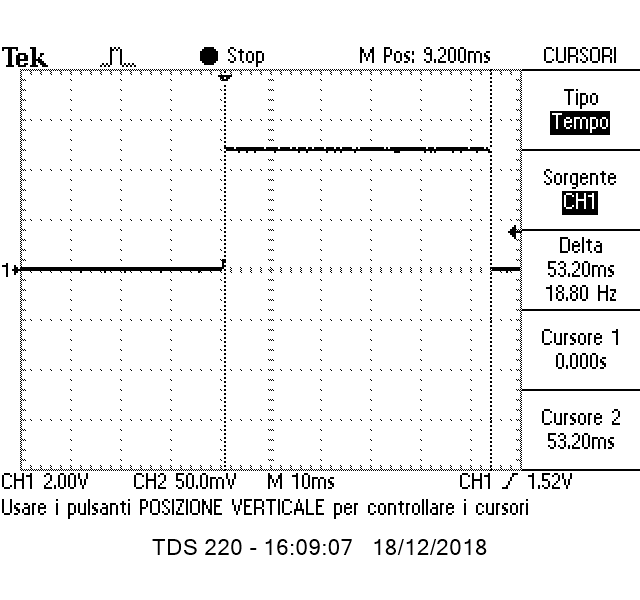
\includegraphics[width=0.8\linewidth]{verificaosc}
	\captionof{figure}{Onda quadra visualizzata sull'oscilloscopio}
	\label{fig:verifiche_osc}
	\end{center}
\end{Figure}

\begin{Figure}
	\begin{center}
	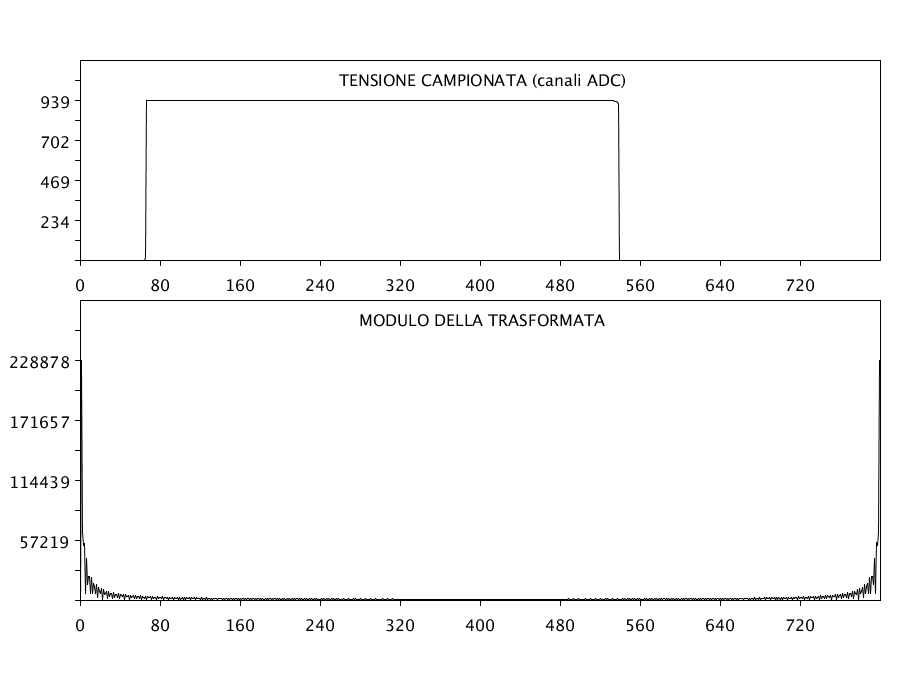
\includegraphics[width=\linewidth]{verifica}
	\captionof{figure}{Onda quadra campionata da Arduino con il programma \emph{Processing}}
	\label{fig:verifiche_ADC}
	\end{center}
\end{Figure}


%==================================================
%             SEGNALE ANALOGICO SENZA RUMORE
%==================================================
\section{Segnale analogico in assenza di rumore}
Si campionano e si studiano in frequenza dei segnali analogici prodotti dal generatore di funzioni in assenza di rumore artificiale.
\subsection{Segnale sinusoidale}
Si campiona digitalmente un segnale sinusoidale (variabile tra $0$ e \SI{4.88 \pm 0.14}{V}) analogico in ingresso a frequenze $f_1 = \SI{212 \pm 6}{\hertz}, \; f_2 = \SI{4.3 \pm 0.1}{\kilo\hertz}$ e infine $f_3 = \SI{6.2 \pm 0.2}{\kilo\hertz}$, quest'ultima volutamente superiore al limite dettato dalla frequenza di Nyquist (\ref{eq:Nyquist}) per poter apprezzare i fenomeni di \emph{aliasing}; le frequenze sono misurate con l'oscilloscopio, collegando direttamente il segnale dal generatore di funzioni al canale \texttt{CH1} dello strumento.

Si riportano in Figura \ref{fig:sin200} e in Figura \ref{fig:sin200osc} il segnale a frequenza $f_1$ campionato da Arduino con la sua trasformata di Fourier discreta e l'istantanea dell'oscilloscopio per questa configurazione, rispettivamente. Sull'asse delle ascisse del grafico della trasformata sono riportate le frequenze di Fourier tenendo presente la relazione~(\ref{eq:ktof}) che lega la frequenza all'indice $k$.

\begin{Figure}
	\begin{center}
	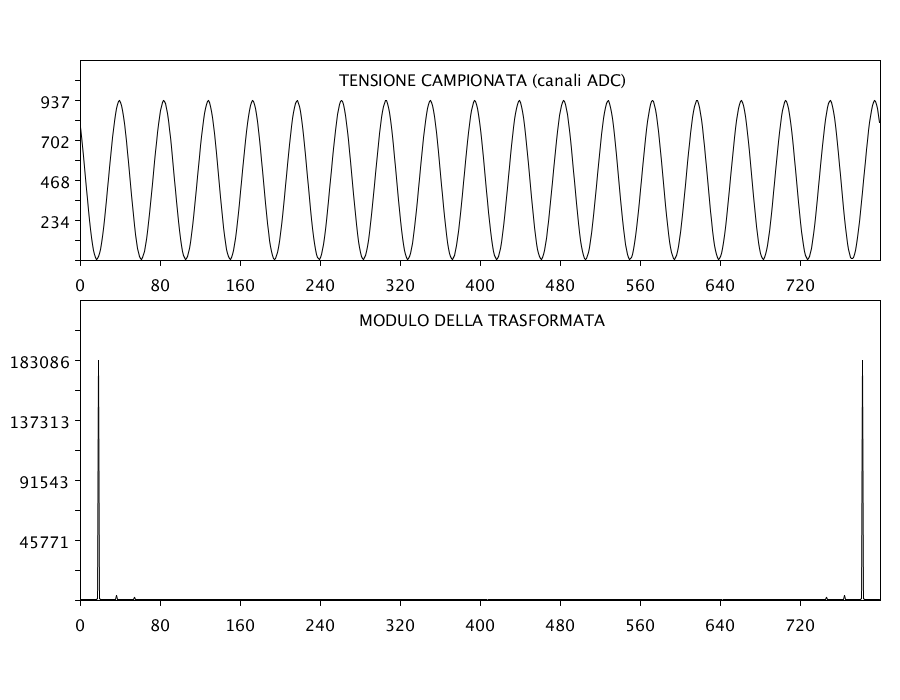
\includegraphics[width=\linewidth]{sin200}
	\captionof{figure}{Segnale sinusoidale analogico a frequenza $f_1$ e sua trasformata di Fourier realizzata con Arduino}
	\label{fig:sin200}
	\end{center}
\end{Figure}
\begin{Figure}
	\begin{center}
	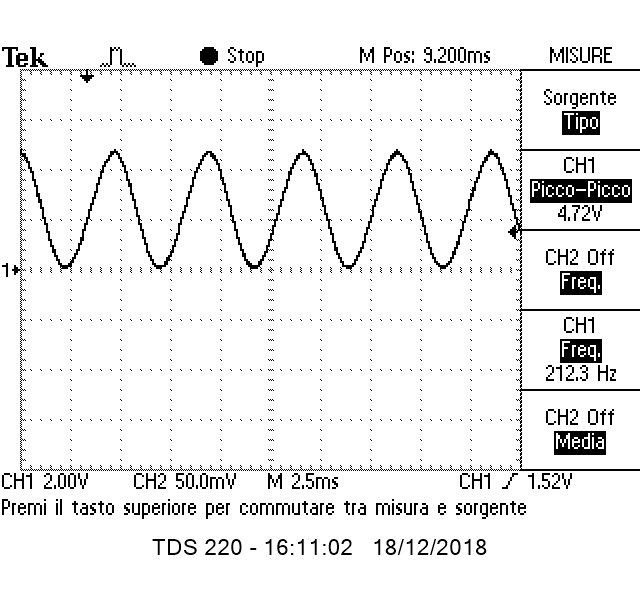
\includegraphics[width=0.8\linewidth]{sin200osc}
	\captionof{figure}{Istantanea dell'oscilloscopio per il segnale sinusoidale a frequenza $f_1$}
	\label{fig:sin200osc}
	\end{center}
\end{Figure}
\begin{Figure}
	\begin{center}
	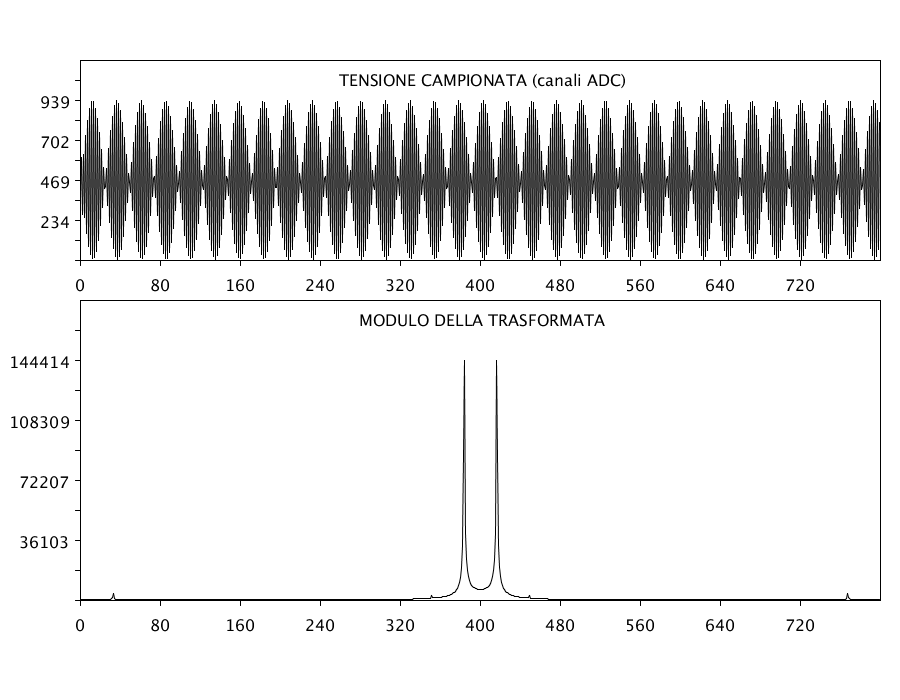
\includegraphics[width=\linewidth]{sin42}
	\captionof{figure}{Segnale sinusoidale analogico a frequenza $f_2$ e sua trasformata di Fourier realizzata con Arduino}
	\label{fig:sin42}
	\end{center}
\end{Figure}
\begin{Figure}
	\begin{center}
	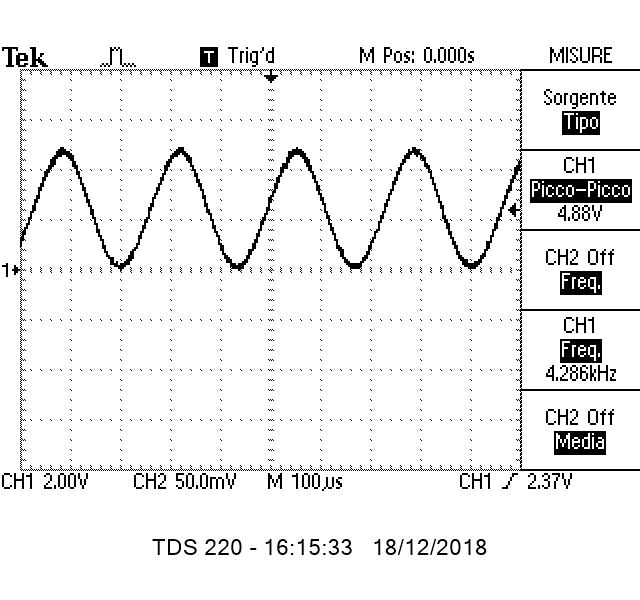
\includegraphics[width=0.8\linewidth]{sin42osc}
	\captionof{figure}{Istantanea dell'oscilloscopio per il segnale sinusoidale a frequenza $f_2$}
	\label{fig:sin42osc}
	\end{center}
\end{Figure}

Come da previsione teorica, la trasformata ha un picco in corrispondenza di $k=18$, dunque ad una frequenza $f_1^\text{(exp)} = \SI{199.8 \pm 0.6}{\Hz}$, compatibile con la frequenza $f_1$ del segnale in ingresso, essendo questo sinusoidale ed essendo lontani dalla frequenza di Nyquist; inoltre, è visibile anche in questo caso il picco simmetrico a $2f_N - f_1^\text{(exp)}$.

Si ripete dunque il campionamento per il segnale sinusoidale a frequenza $f_2$, prossima alla frequenza di Nyquist, e si riportano in Figura \ref{fig:sin42}, \ref{fig:sin42osc} i grafici della tensione in funzione del tempo e della trasformata di Fourier e uno screenshot dell'oscilloscopio. In questo caso, nel grafico dell'acquisizione con l'ADC, sono visibili i battimenti, dovuti alla frequenza molto prossima del segnale campionato e del suo simmetrico con frequenza negativa\footnote{Si ricorda che, poiché il segnale è reale, devono apparire sia la sua frequenza $f$ sia $-f$ per dar conto dell'assenza della parte immaginaria del segnale ricostruito a partire dalla trasformata.}. Dal grafico della trasformata si individua un picco in corrispondenza di $k = 384$, ossia della frequenza $f_2^\text{(exp)} = \SI{4.26 \pm 0.13}{\kilo\Hz}$, compatibile con quella del segnale in ingresso $f_2$.

\begin{Figure}
	\begin{center}
	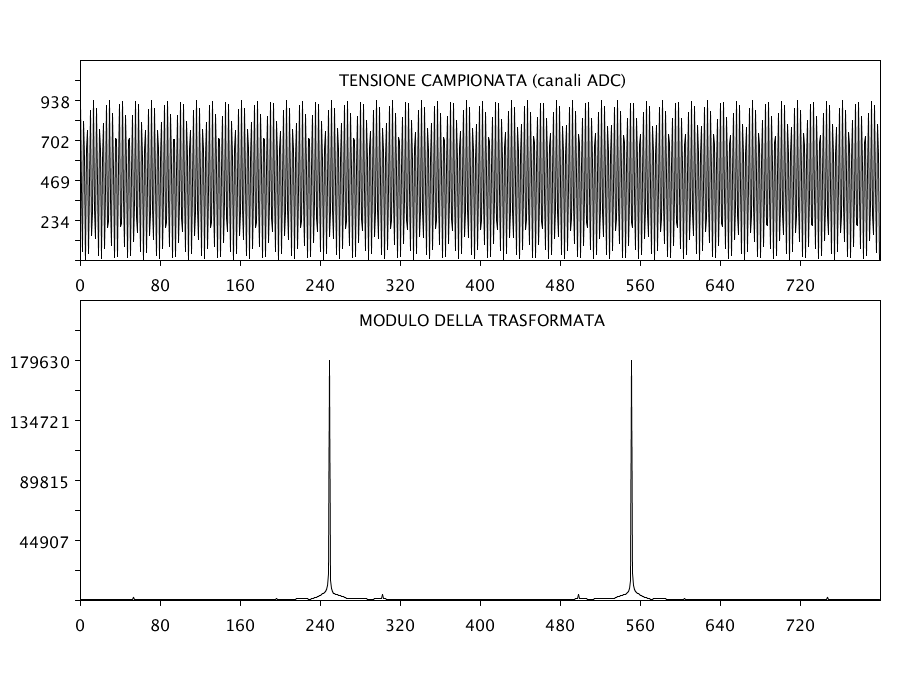
\includegraphics[width=\linewidth]{sin6}
	\captionof{figure}{Segnale sinusoidale analogico a frequenza $f_3$ e sua trasformata di Fourier realizzata con Arduino}
	\label{fig:sin6}
	\end{center}
\end{Figure}
\begin{Figure}
	\begin{center}
	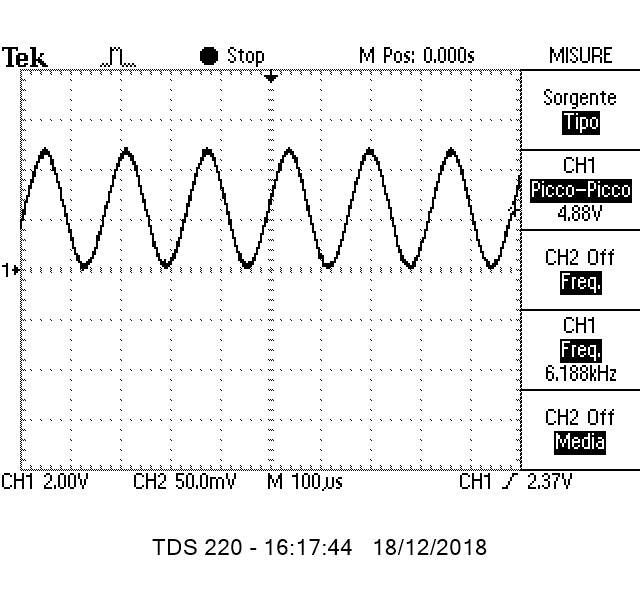
\includegraphics[width=0.8\linewidth]{sin6osc}
	\captionof{figure}{Istantanea dell'oscilloscopio per il segnale sinusoidale a frequenza $f_3$}
	\label{fig:sin6osc}
	\end{center}
\end{Figure}

Infine si campiona il segnale sinusoidale a frequenza $f_3 > f_N$, per il quale si prevede di osservare il fenomeno dell'\emph{aliasing}, come previsto dal Teorema di Nyquist-Shannon. Si riportano in Figura~\ref{fig:sin6} e \ref{fig:sin6osc} il grafico della tensione campionata e della sua trasformata di Fourier e un'istantanea dell'oscilloscopio. Si individua il picco della trasformata in corrispondenza di $k = 249$, ossia alla frequenza $f_3^\text{(alias)} = \SI{2.76 \pm 0.01}{\kilo\Hz}$, che è diversa da quella del segnale $f_3$ misurata dall'oscilloscopio. La frequenza compatibile con quest'ultima è però la simmetrica rispetto a $f_N$, ossia $f_3^\text{(exp)} = \SI{6.11 \pm 0.02}{\kilo\Hz}$ (a $k=551$), che è collocata proprio in $2f_N-f_3^\text{(alias)}$.



Data la medesima procedura sperimentale seguita per gli ultimi due segnali sinusoidali, si procede a compiere $6$ misure analoghe, $3$ a frequenza $f<f_N$ e $3$ a frequenza $f>f_N$. I risultati sono riportati in Tabella~\ref{tab:misure_sin}.

\begin{table*}
\captionof{table}{Campionamento di segnali sinusoidali a $f<f_N$ e $f>f_N$}
\label{tab:misure_sin}
\centering
\begin{tabular}{c|c|c|c|c}
$f$ [\SI{}{\kilo\Hz}] & $k$ & $f^\text{(exp)}$ [\SI{}{\kilo\Hz}] & $k_\text{alias}$ & $f^\text{(alias)}$ [\SI{}{\kilo\Hz}] \\
$(\pm 3\%)$ & & $(\pm 0.3\%)$ &  & $(\pm 0.3\%)$  \\ 
\hline
0.740 &			66  & 0.732	 & 	734 & 8.14 	\\
1.57 & 			141 & 1.56   & 659	& 7.31 \\
3.64 & 			326 & 3.62	 & 474 	& 5.26  \\  
6.9  &			174 & 1.93	 & 626  & 6.94 \\
7.7  & 			116 & 1.29	 & 684  & 7.59 \\
8.4  &			47  & 0.52	 & 753  & 8.35 \\			 
\hline
\end{tabular}
\end{table*}

Si osserva che la frequenza del segnale è compatibile con $f^\text{(exp)}$ per i segnali a $f<f_N$, e con $f^\text{(alias)}$ per quelli a $f>f_N$.

\subsection{Onda quadra}
Si invia al pin \texttt{A3} di Arduino un'onda quadra variabile tra $0$ e \SI{4.96 \pm 0.15}{V} a frequenza $f = \SI{457 \pm 13}{\Hz}$, misurata con l'oscilloscopio. Si effettua il campionamento della stessa (e si è scelta $f<f_N$ appositamente), e si riportano in Figura~\ref{fig:quadra} e~\ref{fig:quadraosc} la tensione in funzione del tempo e la trasformata di Fourier e uno screenshot dell'oscilloscopio. 

\begin{Figure}
	\begin{center}
	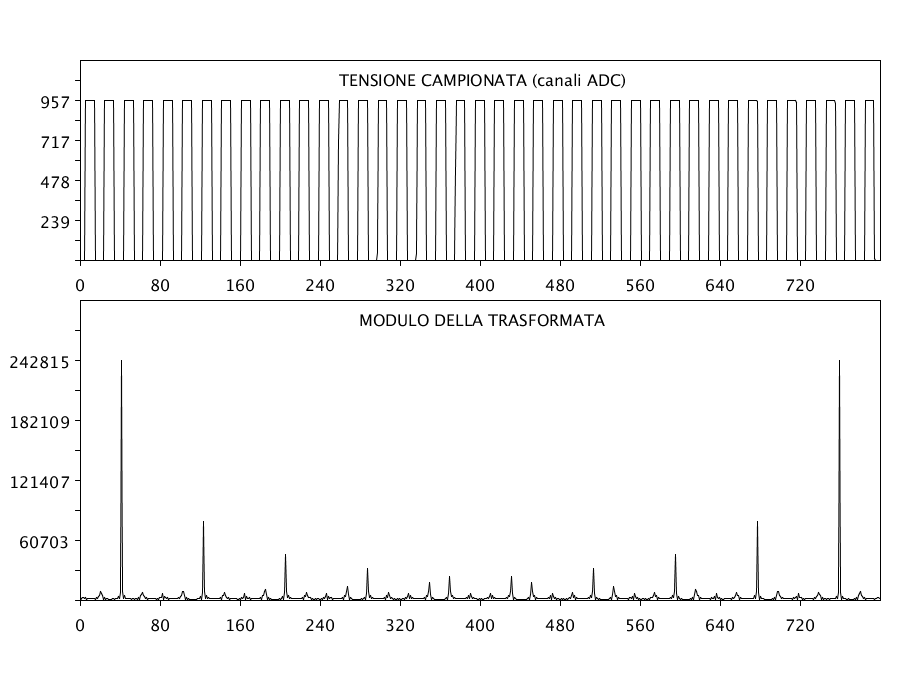
\includegraphics[width=\linewidth]{quadra}
	\captionof{figure}{Onda quadra e sua trasformata di Fourier realizzata con Arduino}
	\label{fig:quadra}
	\end{center}
\end{Figure}
\begin{Figure}
	\begin{center}
	\includegraphics[width=0.8\linewidth]{quadraosc}
	\captionof{figure}{Istantanea dell'oscilloscopio per l'onda quadra}
	\label{fig:quadraosc}
	\end{center}
\end{Figure}
\begin{Figure}
	\begin{center}
	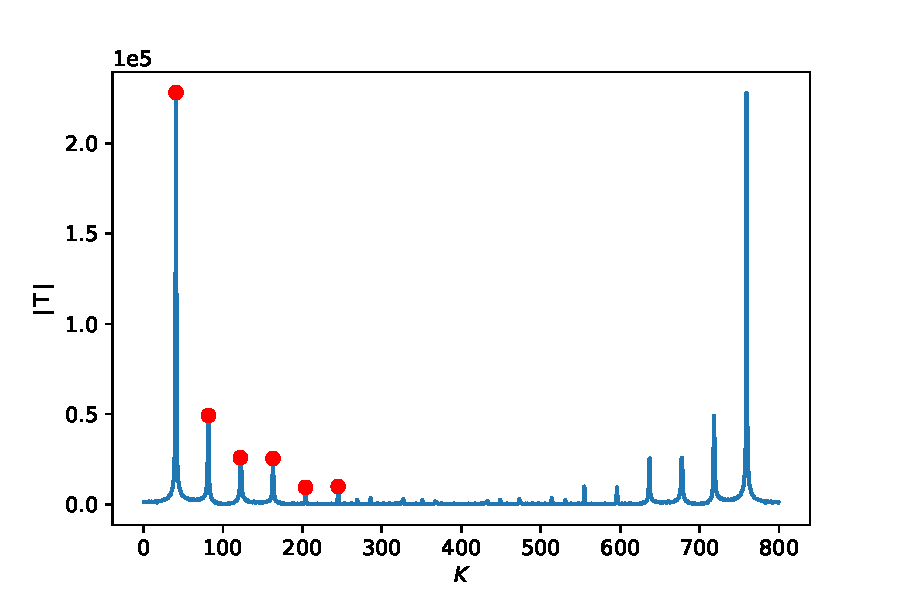
\includegraphics[width=\linewidth]{rumore_analisi.pdf}
	\captionof{figure}{Massimi dello spettro dell'onda quadra individuati dall'algoritmo, in ordinata i moduli della trasformata di Fourier si intendono moltiplicati per $10^5$}
	\label{fig:armoniche_quadra}
	\end{center}
\end{Figure}

Si individuano sul grafico della trasformata i picchi relativi alle armoniche dispari dello sviluppo in serie di Fourier dell'onda quadra, che si ricorda essere
\[
V(t) = V_0 \sum_{n=0}^{\infty} \frac{4}{\pi(2n+1)} \sin(2\pi f t(2n+1)), 
\]
e si nota che si hanno frequenze inferiori a quella di Nyquist fino alla nona armonica, ossia per $(2n+1) = 9$. Si riportano dunque in Tabella~\ref{tab:armoniche_quadra} le frequenze teoriche dello sviluppo in serie dell'onda quadra, $f_n = (2n+1)f$, e le corrispondenti frequenze sperimentali individuate dai picchi. Esse sono state individuate mediante un algoritmo in \texttt{Python}, il cui risultato è evidenziato nel grafico di Figura~\ref{fig:armoniche_quadra}.




Si interpone quindi tra il segnale di onda quadra e Arduino un filtro VCVS \emph{Butterworth} passa basso\footnote{Per i dettagli del filtro utilizzato si rimanda alla relazione dell'esperienza numero 5.}, al fine di eliminare le frequenze superiori a quella di Nyquist, in modo da ottenere nello spettro solo le armoniche fino a $(2n+1)=9$. Si riporta in Figura~\ref{fig:quadraFiltroOsc} lo screenshot dell'oscilloscopio per questa configurazione, nel quale è visibile in basso l'onda quadra in ingresso e in alto l'onda filtrata in uscita, la quale mostra la mancanza delle armoniche maggiori. In Figura~\ref{fig:quadraFiltro} sono riportati i grafici del campionamento e del modulo della trasformata ottenuti con Arduino: si osserva come solo le frequenze inferiori a quella di Nyquist sono presenti nello spettro.
Analogamente a quanto fatto precedentemente, si individuano i picchi e si riportano i risultati in Tabella \ref{tab:armoniche_quadra_filtro}: si osserva che le armoniche sono ancora compatibili con quelle teoriche e che per frequenze superiori a quella di taglio (di circa $\SI{1}{\kilo\hertz}$) i moduli della trasformata di Fourier vengono notevolmente attutiti.

In Figura \ref{fig:quadraFiltro} sono visibili dei picchi in corrispondenza di frequenze inesistenti nel caso non filtrato, si ritiene che ciò sia dovuto all'amplificazione generata dal filtro: infatti l'onda quadra oscillante tra $0$ e $V_\text{max}$ è stata ottenuta aggiungendo manualmente un offset al generatore di funzioni, molto probabilmente l'onda oscillava in realtà tra un valore negativo in modulo vicino a $0$ e $V_\text{max}$, questo valore negativo è stato amplificato dal filtro e dunque l'onda risulta tagliata in maniera non più trascurabile\footnote{Perché, si ricorda, l'Arduino misura solamente tensioni positive.}, come visibile in Figura \ref{fig:quadraFiltroOsc}. Le parti orizzontali, non proprie della funzione originale, generano quelle frequenze impreviste. In tale ottica, nella tabella \ref{tab:armoniche_quadra_filtro} vengono riportati solo i massimi corrispondenti ad armoniche teoricamente corrette.

\begin{Figure}
	\begin{center}
	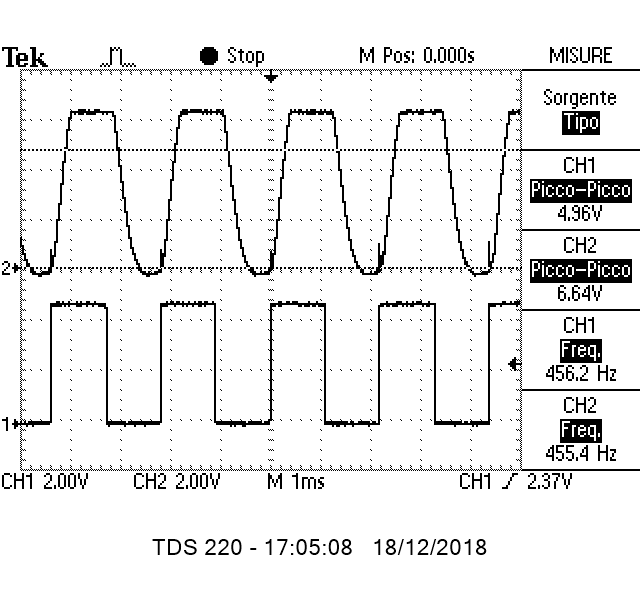
\includegraphics[width=0.8\linewidth]{quadraFiltroOsc}
	\captionof{figure}{Istantanea dell'oscilloscopio per l'onda quadra filtrata}
	\label{fig:quadraFiltroOsc}
	\end{center}
\end{Figure}

\begin{Figure}
	\begin{center}
	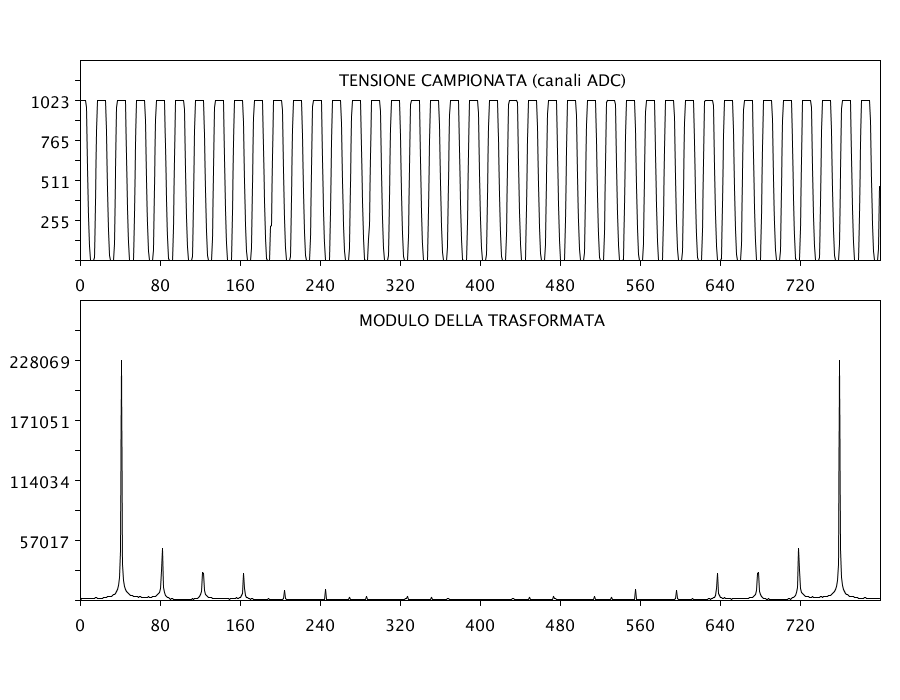
\includegraphics[width=\linewidth]{quadraFiltro}
	\captionof{figure}{Onda quadra filtrata e sua trasformata di Fourier realizzata con Arduino}
	\label{fig:quadraFiltro}
	\end{center}
\end{Figure}

\begin{table*}
\captionof{table}{Spettro dell'onda quadra, armoniche $f_n<f_N$}
\label{tab:armoniche_quadra}
\centering
\begin{tabular}{c|c|c|c|c}
$2n+1$ & $f^\text{(teo)}$ [\SI{}{\kilo\Hz}] & $k$ & $f^\text{(exp)}$ [\SI{}{\kilo\Hz}] & $\vert T \vert$\ \\
 & & & $(\pm 3\%)$ &   \\ 
\hline		
1 		&	0.457	& 	41		&	0.455 	& 	$242.8\times10^3$	\\
3		&	1.37		& 	123		&	1.36		& 	$79.8\times10^3$\\
5		&	2.29		& 	205		&	2.27		& 	$46.5\times10^3$\\
7		&	3.20		& 	287		&	3.18		& 	$31.8\times10^3$\\
9 		&	4.11		& 	369		&	4.09		& 	$23.4\times10^3$\\
\hline
\end{tabular}
\end{table*}

\begin{table*}
\captionof{table}{Spettro dell'onda quadra filtrata, armoniche $f_n<f_N$}
\label{tab:armoniche_quadra_filtro}
\centering
\begin{tabular}{c|c|c|c|c}
$2n+1$ & $f^\text{(teo)}$ [\SI{}{\kilo\Hz}] & $k$ & $f^\text{(exp)}$ [\SI{}{\kilo\Hz}] & $\vert T \vert$\ \\
 & & & $(\pm 3\%)$ &   \\ 
\hline		
1 		&	0.457	& 	41		&	0.455 	& 	$228.1\times10^3$	\\
3		&	1.35		& 	122		&	1.36		& 	$25.9\times10^3$\\
5		&	2.26		& 	204		&	2.27		& 	$9.48\times10^3$\\
\hline
\end{tabular}
\end{table*}




%==================================================
%             STUDIO DEL RUMORE
%==================================================
\section{Studio del rumore}
Si genera artificialmente un rumore bianco, utilizzando un transistor in regime di \emph{breakdown}, e lo si analizza in frequenza. Essendo il segnale a media nulla, e potendo noi misurare solo tensioni positive, si somma al rumore una tensione continua di circa $\SI{1}{V}$ attraverso un sommatore a tre ingressi: in questo modo si riesce a campionare l'intera oscillazione del rumore. Si riporta in Figura \ref{fig:rumoreOsc} un'istantanea dell'oscilloscopio del rumore generato.

\begin{Figure}
	\begin{center}
	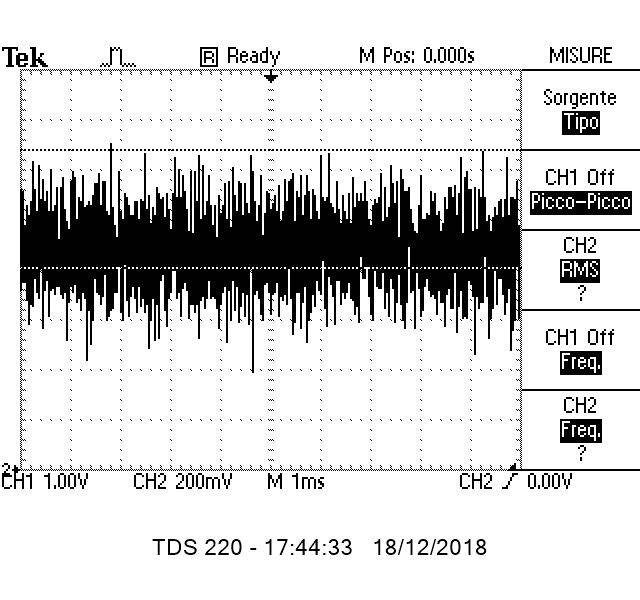
\includegraphics[width=0.8\linewidth]{rumoreOsc}
	\captionof{figure}{Istantanea dell'oscilloscopio del rumore bianco generato artificialmente e sommato ad una tensione continua}
	\label{fig:rumoreOsc}
	\end{center}
\end{Figure}

In Figura \ref{fig:rumore} è riportato il campionamento digitale del rumore e la sua analisi in frequenza: è visibile una frequenza parassita predominante non aleatoria, che cioè rimaneva costante ripetendo la misura. Dopo alcuni minuti tale frequenza, ancora presente, è diventata meno predominante, un esempio è riportato in Figura \ref{fig:rumoreBuono}.

\begin{Figure}
	\begin{center}
	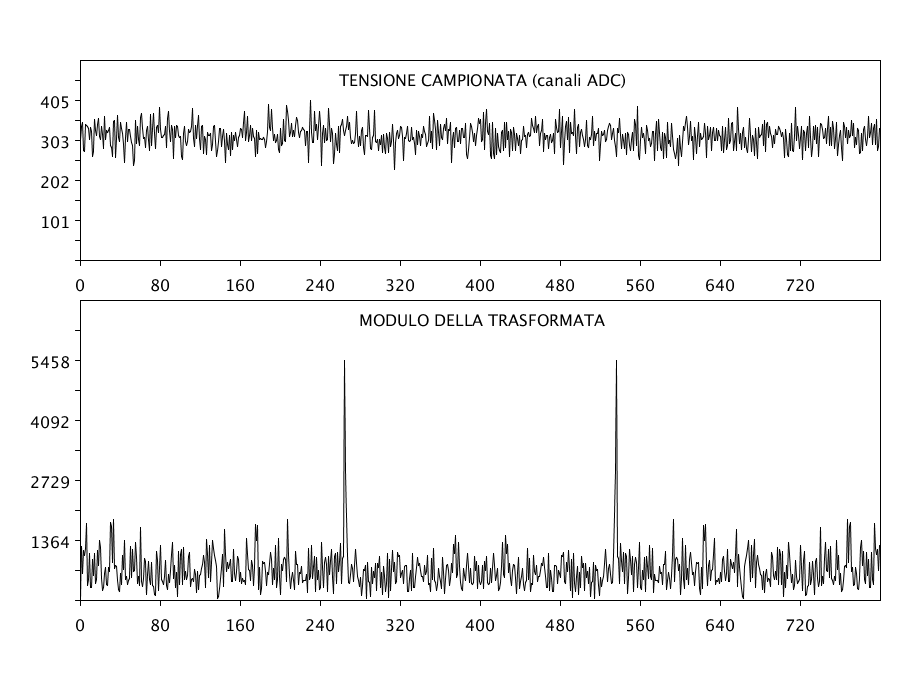
\includegraphics[width=\linewidth]{rumore}
	\captionof{figure}{Campionamento digitale e analisi in frequenza di un rumore bianco artificiale, è visibile una frequenza parassita predominante}
	\label{fig:rumore}
	\end{center}
\end{Figure}
\begin{Figure}
	\begin{center}
	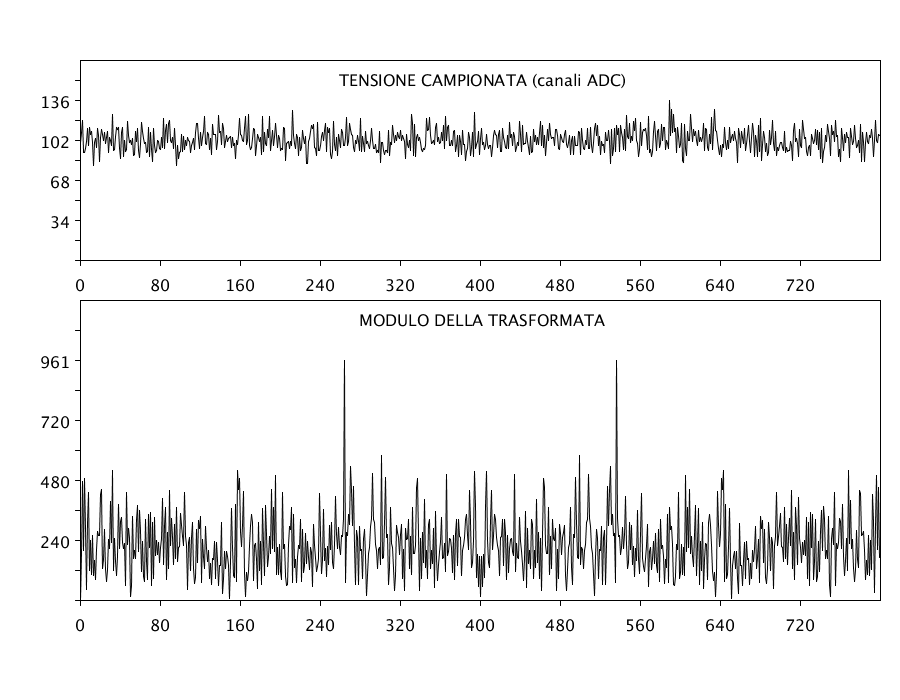
\includegraphics[width=\linewidth]{rumoreBuono}
	\captionof{figure}{Campionamento digitale e analisi in frequenza di un rumore bianco artificiale, misura fatta a distanza di pochi minuti da quella in figura precedente, la frequenza parassita risulta ancora presente ma meno dominante}
	\label{fig:rumoreBuono}
	\end{center}
\end{Figure}

Essendo il rumore di natura aleatoria, lo studio in frequenza viene fatto su un campione di 5 misure. Si riporta in Figura \ref{fig:studioRumore} la distribuzione dei valori quadratici medi dei moduli della trasformata di Fourier per le diverse frequenze dello sviluppo, ossia
\[
S(k) = \sqrt{\frac{\sum_{m=1}^5\abs{X_m(k)}^2}{M}} 
\]
Si vede un andamento circa uniforme delle medie, in accordo con la definizione di rumore bianco. È inoltre ben distinguibile la frequenza parassita che, per quanto sia diminuita in intensità rispetto alla prima misura fatta, rimane comunque presente.
\begin{Figure}
	\begin{center}
	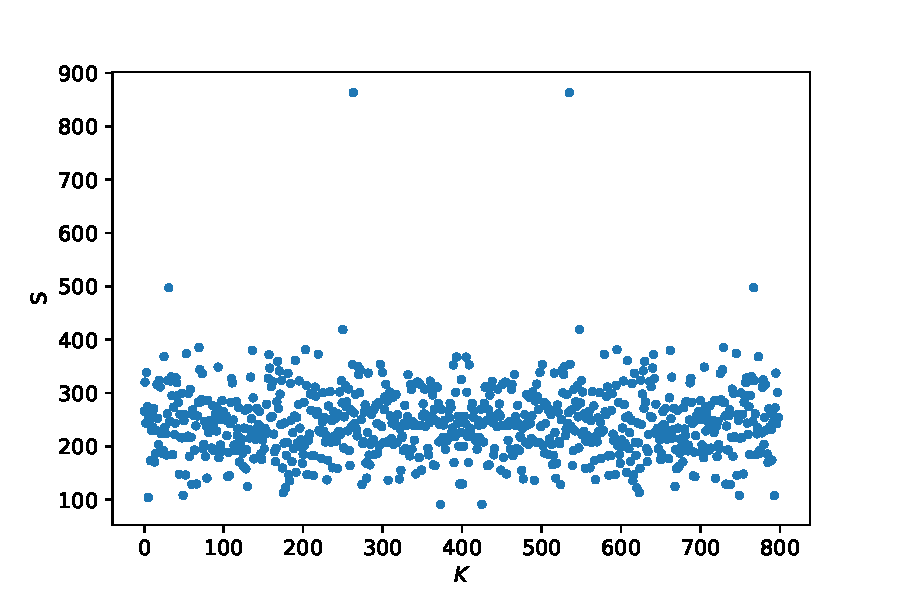
\includegraphics[width=\linewidth]{studioRumore}
	\captionof{figure}{Distribuzione media delle armoniche di cinque campioni di rumore, si distingue un'armonica predominante su un fondo di rumore bianco}
	\label{fig:studioRumore}
	\end{center}
\end{Figure}

Si collega dunque l'uscita del sommatore al filtro VCVS passa basso discusso in precedenza e si ripete l'analisi in frequenza. Si riporta in Figura \ref{fig:rumoreFiltroOsc} un'istantanea dell'oscilloscopio del rumore filtrato, è evidente l'attenuazione dovuta all'abbattimento delle frequenze più elevate. L'analisi più dettagliata è riportata in Figura \ref{fig:rumoreFiltro} mentre la media su cinque campioni è proposta in Figura \ref{fig:studioRumoreFiltro}: in quest'ultima è ben visibile l'effetto del filtro passa basso sulle componenti del rumore, consistente in un picco attorno alla frequenza di taglio del filtro e un andamento decrescente fino alla frequenza di Nyquist. 
\begin{Figure}
	\begin{center}
	\includegraphics[width=0.8\linewidth]{rumoreFIltroOsc}
	\captionof{figure}{Istantanea dell'oscilloscopio del rumore bianco filtrato con un passa basso, è evidente l'attenuazione rispetto al rumore non filtrato}
	\label{fig:rumoreFiltroOsc}
	\end{center}
\end{Figure}

È altresì visibile come il valore di $S$ sia inferiore di un ordine di grandezza rispetto al caso non filtrato, conseguenza dell'eliminazione da parte del filtro delle alte frequenze, responsabili dell'\emph{aliasing}. Tuttavia è bene ricordare che non si possa fare un confronto diretto tra i valori, dal momento che il filtro, come già evidenziato in precedenza, ha un guadagno non trascurabile.

\begin{Figure}
	\begin{center}
	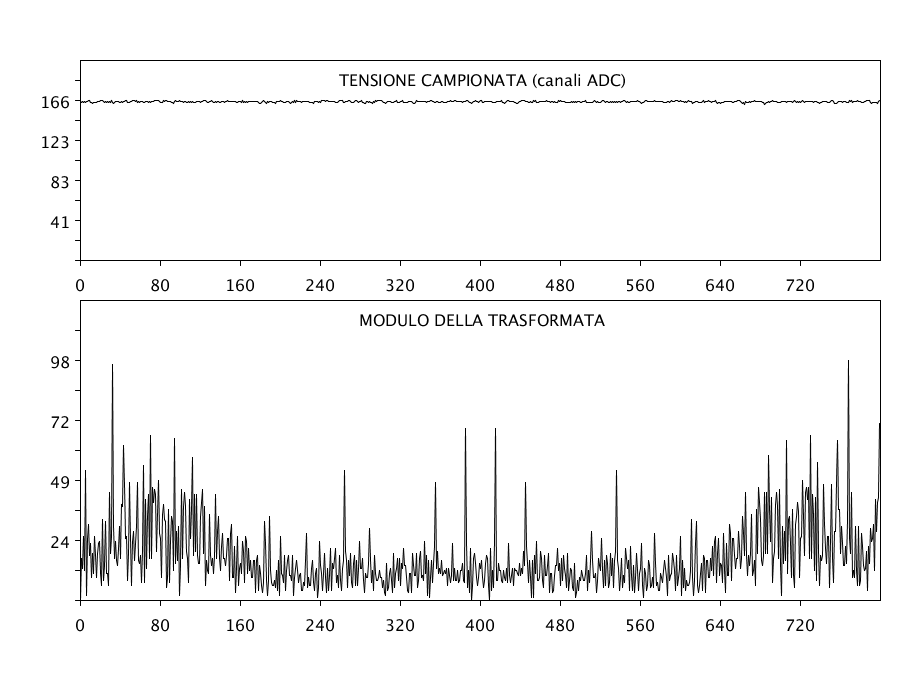
\includegraphics[width=\linewidth]{rumoreFiltro}
	\captionof{figure}{Campionamento digitale e analisi in frequenza di un rumore bianco artificiale filtrato con un passa basso}
	\label{fig:rumoreFiltro}
	\end{center}
\end{Figure}
\begin{Figure}
	\begin{center}
	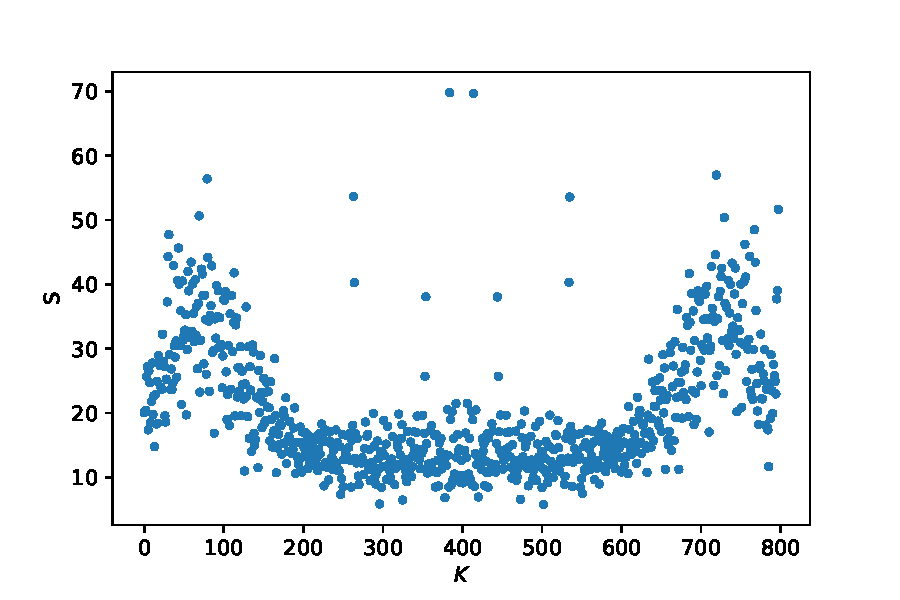
\includegraphics[width=\linewidth]{studioRumoreFiltrato}
	\captionof{figure}{Distribuzione media delle armoniche di cinque campioni di rumore}
	\label{fig:studioRumoreFiltro}
	\end{center}
\end{Figure}


%==================================================
%             SEGNALE IMPULSIVO
%==================================================
\section{Studio di un segnale impulsivo}
Si genera un segnale impulsivo prelevando la tensione in un circuito RC ai capi di un condensatore parzialmente caricato con un semiperiodo di un'onda quadra prodotto da Arduino: l'onda quadra, riportata in Figura \ref{fig:impulsoOsc} e in Figura \ref{fig:impulso}, ha una durata di $t = \SI{2.24 \pm 0.07}{\milli\second}$ ed un'ampiezza di $\SI{3.80 \pm 0.1}{\volt}$, valori misurati con l'oscilloscopio.
I valori nominali dei componenti del circuito RC, misurati con multimetro e ponte, sono $R = \SI{99.8 \pm 0.5}{\kilo\ohm}$ e $C = \SI{101.40 \pm 0.05}{nF}$. Si riesce in questo modo ad ottenere un impulso come quello riportato in Figura \ref{fig:impulsoRC}.

\begin{Figure}
	\begin{center}
	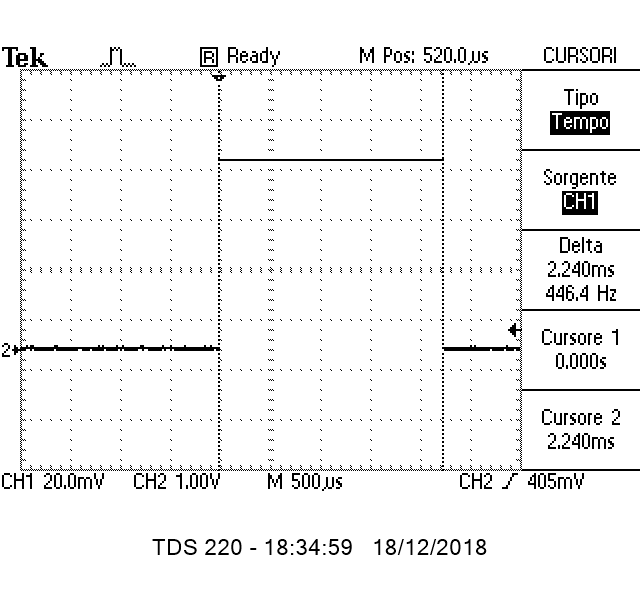
\includegraphics[width=0.7\linewidth]{impulsoOsc}
	\captionof{figure}{Istantanea dell'oscilloscopio dell'onda quadra prodotta da Arduino}
	\label{fig:impulsoOsc}
	\end{center}
\end{Figure}

\begin{Figure}
	\begin{center}
	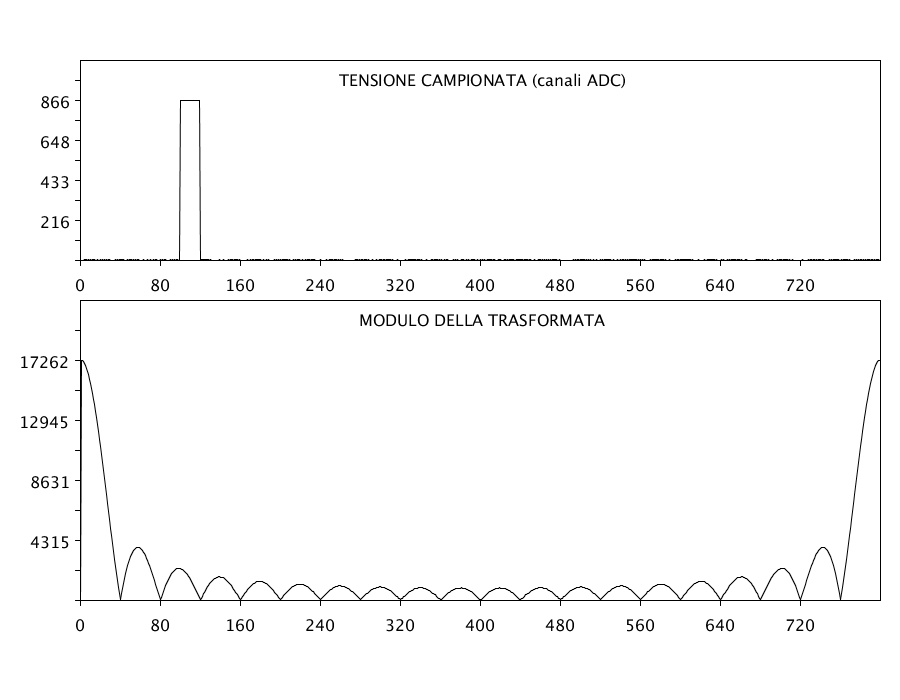
\includegraphics[width=0.9\linewidth]{impulso}
	\captionof{figure}{Semiperiodo di un'onda quadra prodotta da Arduino e sua trasformata di Fourier}
	\label{fig:impulso}
	\end{center}
\end{Figure}

\begin{Figure}
	\begin{center}
	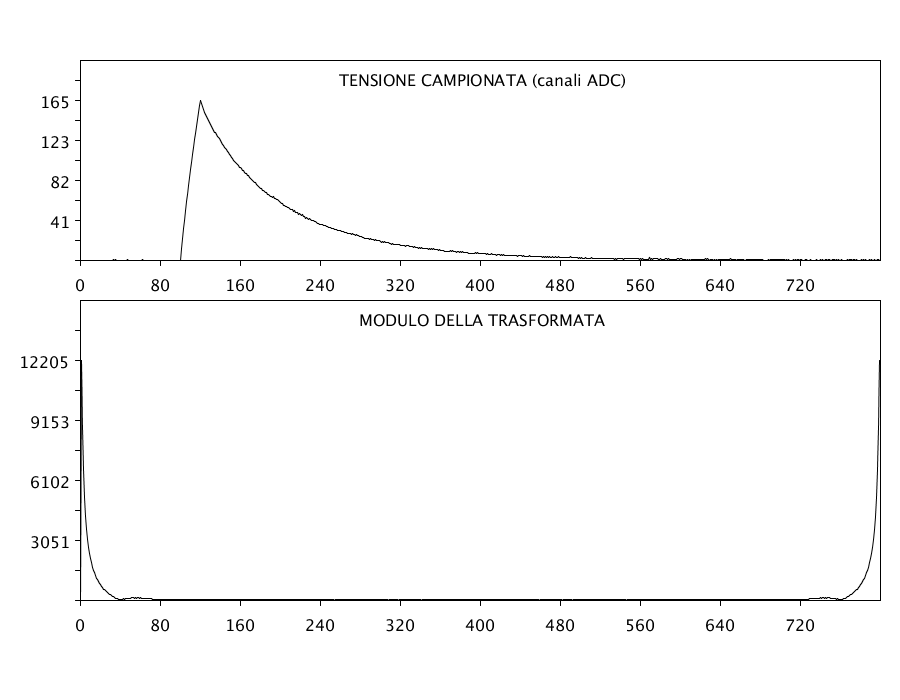
\includegraphics[width=0.9\linewidth]{impulsoRC}
	\captionof{figure}{Impulso generato con un circuito RC e un Arduino e sua trasformata di Fourier}
	\label{fig:impulsoRC}
	\end{center}
\end{Figure}

Si nota che l'ampiezza dell'impulso è circa cinque volte più piccola di quella prodotta dall'Arduino, ciò è dovuto al fatto che l'onda quadra non ha durata sufficiente per caricare completamente il condensatore, inoltre l'impulso si discosta dal caso ideale a causa di un tempo di scarica non trascurabile: entrambi questi inconvenienti potrebbero essere ridotti scegliendo un condensatore di capacità inferiore\footnote{Ma non troppo piccola per evitare di caricarlo completamente prima del termine del segnale.}.

\subsection{Impulso in assenza di rumore}
Il segnale impulsivo si mette in ingresso ad un sommatore a tre ingressi, collegando gli altri due ingressi a massa: si ottiene il segnale riportato in Figura \ref{fig:impulsoRCSommatore}.
\begin{Figure}
	\begin{center}
	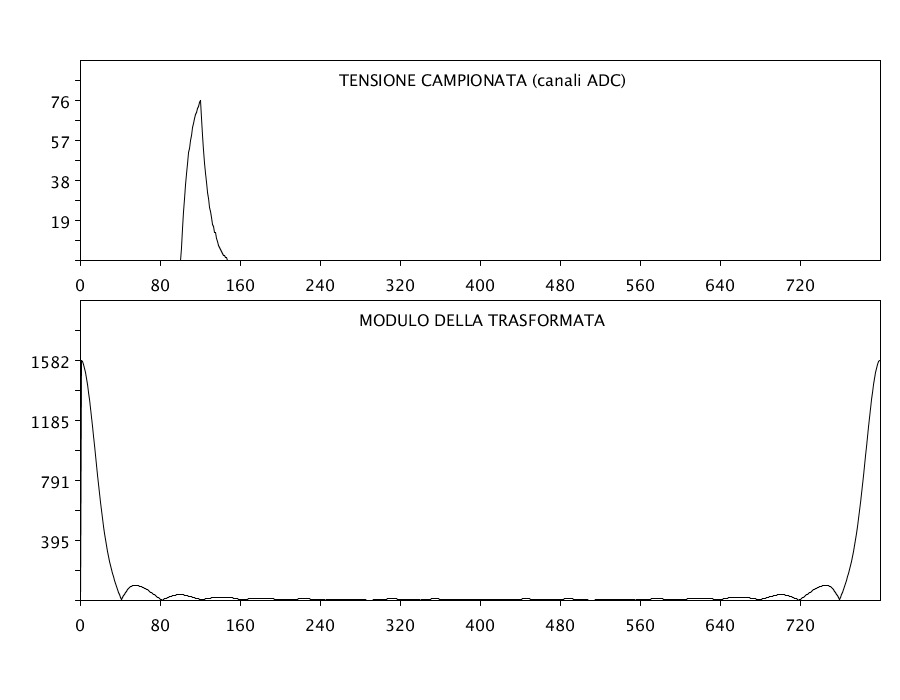
\includegraphics[width=0.9\linewidth]{impulsoRCSommatore}
	\captionof{figure}{Uscita del sommatore con il segnale impulsivo in ingresso}
	\label{fig:impulsoRCSommatore}
	\end{center}
\end{Figure}
Si osserva una distorsione del segnale e un'attenuazione della sua ampiezza. Filtrando l'uscita del sommatore con il filtro VCVS si ottiene il segnale in Figura \ref{fig:impulsoRCSommatoreFiltro}, si osserva che la forma del segnale rimane invariata e che subisce un'amplificazione, coerente con quanto descritto in precedenza.
\begin{Figure}
	\begin{center}
	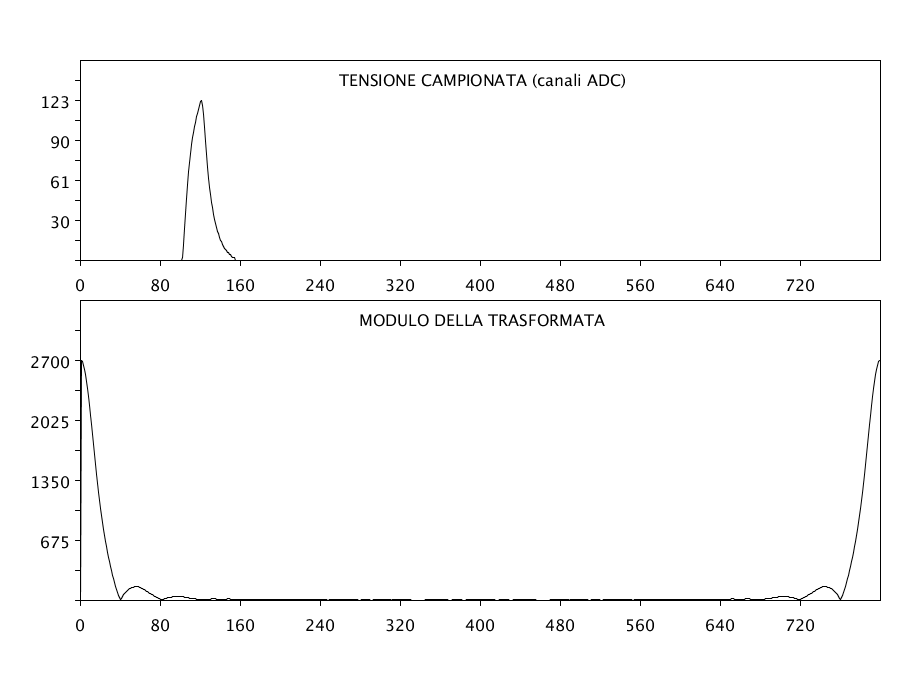
\includegraphics[width=0.9\linewidth]{impulsoRCSommatoreFiltro.png}
	\captionof{figure}{Uscita del sommatore con il segnale impulsivo in ingresso filtrata dal VCVS}
	\label{fig:impulsoRCSommatoreFiltro}
	\end{center}
\end{Figure}

\subsection{Impulso in presenza di rumore}
Utilizzando il circuito sommatore, all'impulso viene aggiunto il rumore artificiale generato come descritto precedentemente. Si ottiene il segnale riportato in Figura \ref{fig:impulsoRCRumore}, dove il picco è appena distinguibile a causa del fatto che la sua ampiezza è confrontabile con quella del rumore; si può comunque individuare il picco della trasformata che caratterizza l'impulso, e un fondo circa uniforme che caratterizza il rumore bianco.
\begin{Figure}
	\begin{center}
	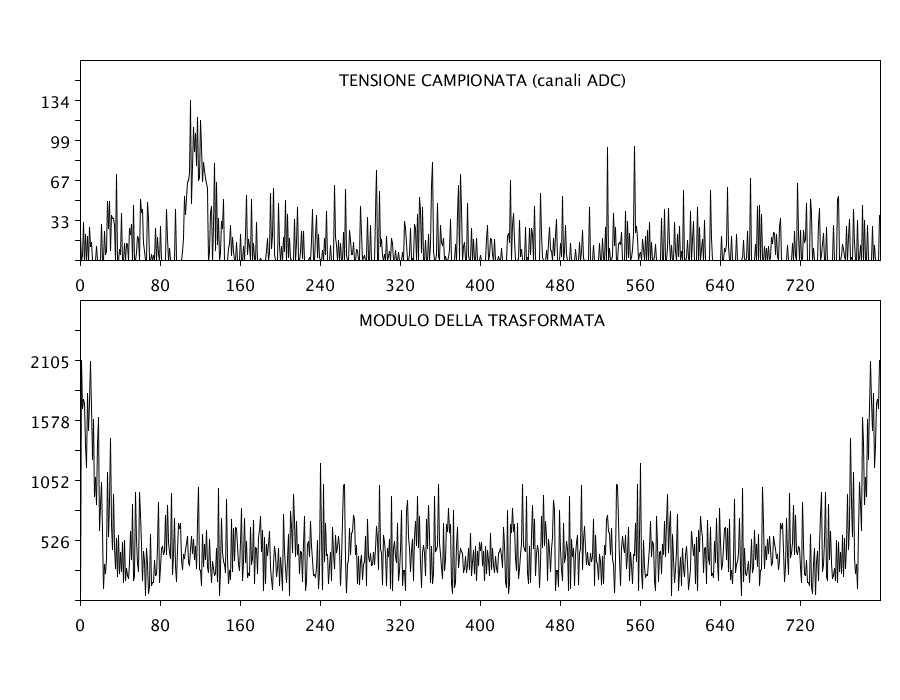
\includegraphics[width=0.9\linewidth]{impulsoRCRumore}
	\captionof{figure}{Segnale impulsivo con rumore bianco}
	\label{fig:impulsoRCRumore}
	\end{center}
\end{Figure}

Filtrando l'uscita del sommatore con un VCVS, tutte le componenti ad alta frequenza vengono attutite e si riesce a \emph{ripulire} notevolmente il segnale impulsivo, come mostrato in Figura \ref{fig:impulsoRCRumoreFiltro}.
\begin{Figure}
	\begin{center}
	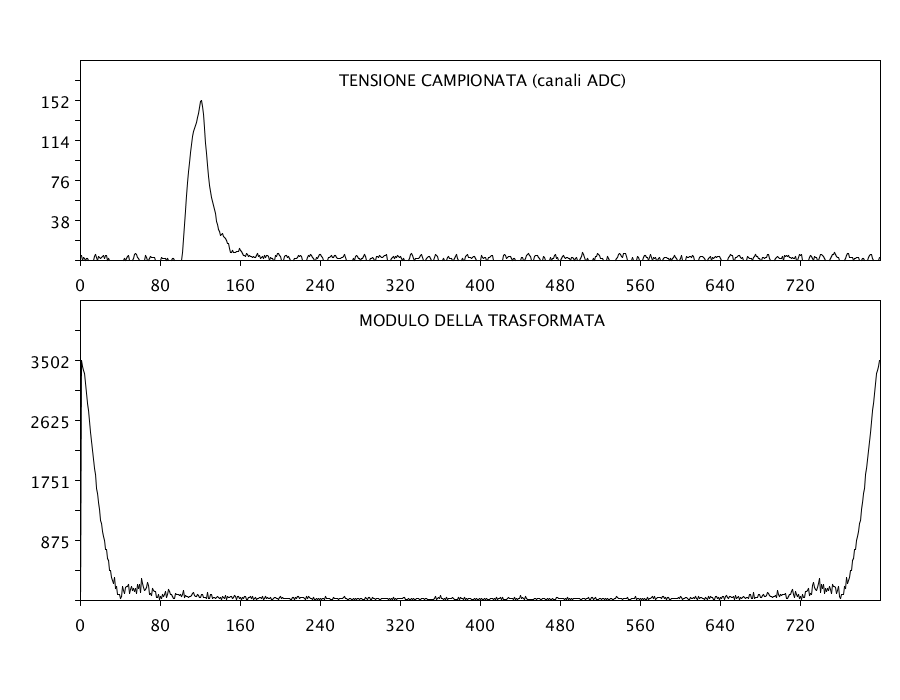
\includegraphics[width=0.9\linewidth]{impulsoRCRumoreFiltro}
	\captionof{figure}{Segnale impulsivo con rumore bianco, filtrato}
	\label{fig:impulsoRCRumoreFiltro}
	\end{center}
\end{Figure}

\end{multicols}
%\newpage
%\section{Appendice}


%ESEMPIO DI CODICE
%\begin{lstlisting}[style=CStyle, caption={Codice per la misura dei tempi di esecuzione della moltiplicazione}, label=lst:moltiplicazione]
%#define MAX 10000
%
%int p, q;
%long unsigned t0, t1;
%
%void setup() {
%	Serial.begin(9600);
%	p=10; 
%}
%
%void loop() { 
%	Serial.print(p);
%	t0 = micros();
%	q = p*10;
%	t1 = micros();
%	p = p+1;	
%	Serial.print(p);
%	Serial.print(" ");
%	Serial.println(t1-t0); //stampa il tempo
%	while (p > MAX) { }; //il programma si arresta quando il numero supera MAX
%	}
%\end{lstlisting}


%ESEMPIO DI FIGURA
%\begin{Figure}
%	\begin{center}
%	\includegraphics[width=\linewidth]{comune.png}
%	\captionof{figure}{Istantanea dell'oscilloscopio per l'amplificatore differenziale, misura di $A_c$}
%	\label{fig:Ac_differenziale}
%	\end{center}
%\end{Figure}


%ESEMPIO DI TABELLA
%\begin{center}
%\captionof{table}{Misure per la stima di $A_c$}
%\label{tab:Ac_differenziale}
%\begin{tabular}{c|c|c|c}
%$f$ [\SI{}{Hz}] & $V_i$ [\SI{}{V}] & $v_o$ [\SI{}{mV}] & $A_c = v_o / V_i$ \\
%\hline
%      149.5 &        3.90 &         11.3 & 2.90e-03 \\
%      222.0 &        3.90 &         11.5 & 2.95e-03 \\
%      281.0 &        3.90 &         11.8 & 3.03e-03 \\
%      359.0 &        3.90 &         11.8 & 3.03e-03 \\
%      461.0 &        3.90 &         12.2 & 3.13e-03 \\
%\hline
%\end{tabular}
%\end{center}



\end{document}